\section{ACCESO}
\subsection{Gráfico de dependencias}
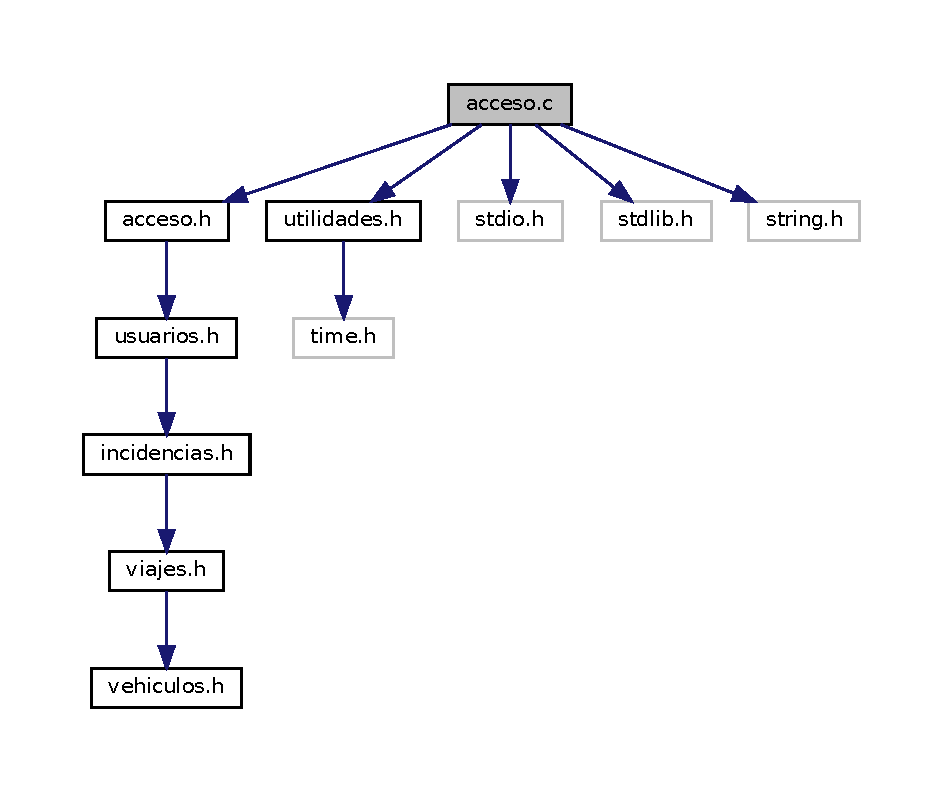
\includegraphics[width=\textwidth, angle=0]{dep/acceso_include.pdf}
\subsection{Funciones}
\begin{itemize}
    \item \cc{int *acceder(vUsuarios *usuarios)}
\end{itemize}
\subsection{Definiciones}
\begin{itemize}
    \item \cc{int *acceder(vUsuarios *usuarios)}
    \begin{itemize}
        \item \textbf{Descripción}
        \begin{itemize}
			\item Comprueba el tipo de usuario (usuario/administrador).
		\end{itemize}
		\item \textbf{Parámetros}
		\begin{itemize}
			\item \cc{usuarios} $\rightarrow$ Referencia al vector user.
		\end{itemize}
		\item \textbf{Devuelve}
		\begin{itemize}
			\item Iésima posición del usuario / -1 si no lo ha encontrado posición 0.
			\item Tipo usuario (0 (admin) / 1 (usuario)) en posición 1.
		\end{itemize}
	\end{itemize}
\end{itemize}
\newpage
